
% Inledningssektionen

I detta projekt skall en robot med förmågan att kartlägga rum som specificeras enligt \cite{coursespec}. Detta ska den göra genom att förflytta sig i rummet (med manuell eller autonom styrning) och skanna med en avståndskänslig laser. Kommandon och resultat skickas till respektive från en extern PC via ett blåtandsgränssnitt.

\begin{figure}[h!]
    \makebox[\textwidth][c]{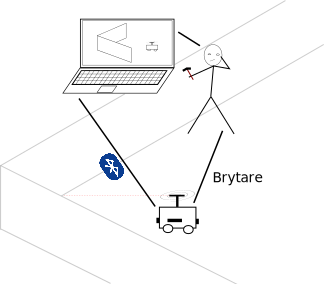
\includegraphics[width=1\textwidth]{overview.png}}
    \caption{Systemet i dess omgivning.}
    \label{fig:overview}
\end{figure}

\noindent
Systemet innehåller fyra kommunicerande datorer, enheter, med egna ansvarsområden och uppgifter:

\begin{itemize}
\item Sensorenhet (se \ref{sec:system1})
\item Styrenhet (se \ref{sec:system2})
\item Kommunikations- och kontrollenhet (se \ref{sec:system3})
\item Extern PC (se \ref{sec:system4})
\end{itemize}

\noindent
Sensorenheten behandlar data från systemets olika sensorer, för att skicka vidare datan på ett mer användbart format med minimala läsfel.

Styrenheten ansvarar för att omvandla högnivåkommandon till lågnivåkommandon och propagera dessa till systemets olika motorer och servos.

Kommunikations- och kontrollenheten är den centrala hjärnan i systemet, som skickar kommandon till de andra enheterna. I det manuella utför den kommandon som kommer ifrån den externa PC:n, och i det autonoma bestämmer den själv bästa tillvägagångssätt för att systemet själv ska kunna kartlägga rummet.

På den externa PC:n finner vi ett användargränssnitt där en människa kan läsa av resultat, avlusningsdata, samt skicka kommandon om roboten befinner sig i det manuella läget.

I figur \ref{fig:modules} beskrivs det grafiskt hur dessa moduler kommunicerar med varandra. Mer detaljerade blockschema finns till varje modul, samt en fullständig översikt i figur \ref{fig:modulesDetailed}.

\begin{figure}[h!]
    \makebox[\textwidth][c]{\includegraphics[width=1\textwidth]{modules.png}}
    \caption{Modulöversikt.}
    \label{fig:modules}
\end{figure}

\noindent
Robotens hårdvara är monterad ovanpå dess chassi, en modell som går under namnet \cite{terminator}. Denna kommer med fyra hjul påmonterade, som används för att roboten ska kunna ta sig runt i rummet. Ett servo till, modell AX-12, monteras på toppen av roboten.

Ovanpå denna monteras den avståndskänsliga lasern LIDAR - systemets främsta vapen vad gäller rumskanning. Ytterligare sensorer hittas på tre av robotens fyra sidor: IR-sensorer för bättre kontroll under körning. Ingen monteras längst fram på chassit, då LIDARn täcker den funktionaliteten då roboten rör på sig.

Ett gyro, modell MLX90609, monteras även i mitten av roboten för att kunna rotera roboten mer precist.

I figur \ref{fig:placement} hittar ni en grafisk beskrivning av hårdvarans placering.

\begin{figure}[h!]
    \makebox[\textwidth][c]{\includegraphics[scale=0.40]{layout_topdown.png}}
    \caption{Placering av hårdvara på robotchassit.}
    \label{fig:placement}
\end{figure}
